\section{Deployment View}
\subsection{Mô tả tổng quan hệ thống}
Triển khai môi trường thực thi vật lý của hệ thống quản lý bãi đỗ xe thông minh HCMUT, minh họa cách thức các thành phần phần mềm được phân bổ và hoạt động trên các thiết bị phần cứng. Hệ thống được thiết kế theo kiến trúc phân tầng bao gồm: 
\begin{itemize}
    \item \textbf{IoT \& Edge Layer (Hạ tầng tại khuôn viên của trường):} Bao gồm các thiết bị cảm biến, camera và bộ điều khiển tại chỗ để thu thập dữ liệu về tình trạng bãi đỗ xe và thực hiện các hành động cơ bản như mở cửa cổng.
    \item \textbf{Client Layer (Ứng dụng người dùng cuối):} Bao gồm các ứng dụng người dùng cuối như ứng dụng di động và trang web để tương tác với hệ thống.
    \item \textbf{Server/Cloud Layer (Cơ sở hạ tầng của hệ thống):} Xử lý nghiệp vụ tập trung và lưu trữ dữ liệu.
    \item \textbf{External Integration Layer (Các hệ thống tích hợp bên ngoài):} Kết nối với các dịch vụ bên ngoài như hệ thống đăng nhập tập trung và hệ thống thanh toán.
\end{itemize}
Việc phân chia này giúp hệ thống đảm bảo tính mở rộng, dễ dàng bảo trì và quản lý luồng dữ liệu hiệu quả từ các thiết bị đầu cuối đến các máy chủ trung tâm.

\subsection{Sơ đồ triển khai hệ thống}
\begin{figure}[H]
    \centering
    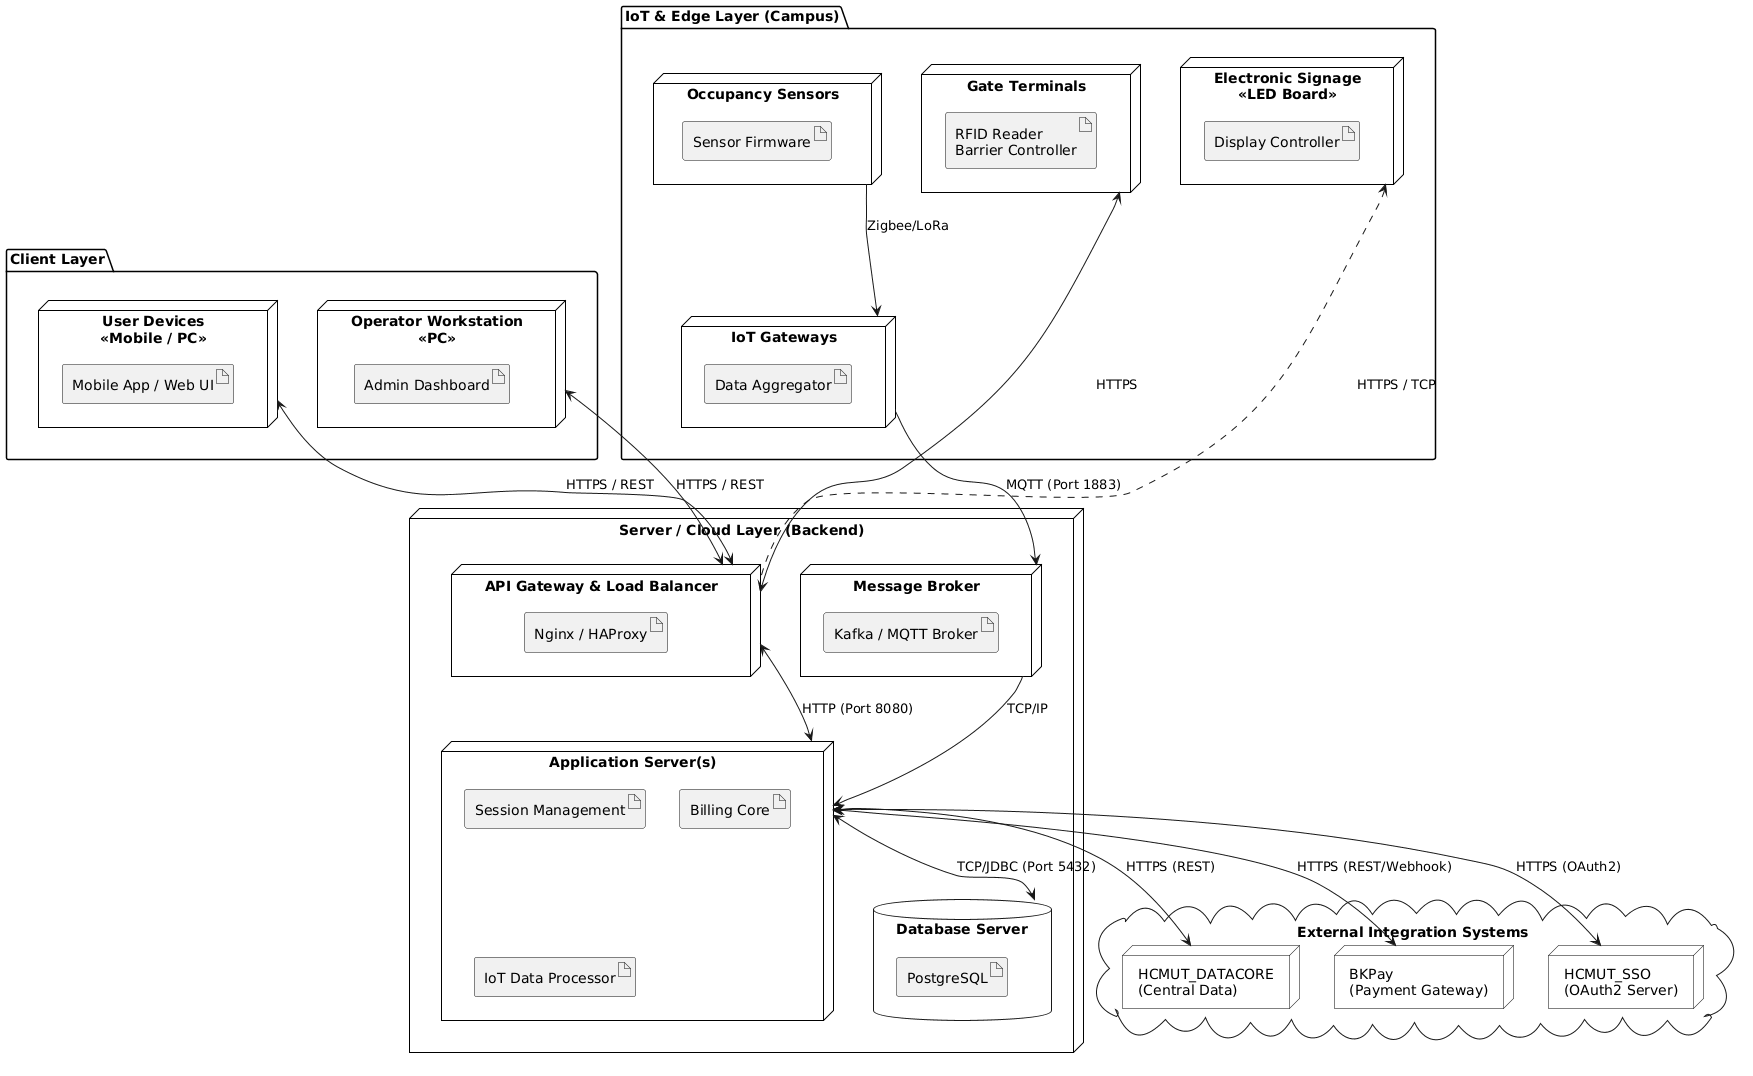
\includegraphics[angle=-90, width=0.5\textheight, keepaspectratio]{../design/deployment_diagram.png}
    \caption{Sơ đồ triển khai hệ thống quản lý bãi đỗ xe thông minh HCMUT}
\end{figure}

\subsection{Thành phần chi tiết}
\subsubsection{IoT \& Edge Layer}
Tầng này bao gồm các thiết bị vật lý được lắp đặt trực tiếp tại các bãi đỗ xe và cổng ra vào của trường đại học.
\begin{itemize}
    \item \textbf{Occupancy Sensors (Cảm biến hiện diện):}
    \begin{itemize}
        \item \textbf{Phần cứng:} Cảm biến siêu âm hoặc từ trường gắn tại mỗi ô đỗ xe.
        \item \textbf{Phần mềm:} Sensor Firmware.
        \item \textbf{Vai trò:} Nhận diện có xe đang đỗ hay không. Gửi tín hiệu (dạng thô) về IoT Gateway thông qua sóng tầm ngắn (Zigbee, LoRa, hoặc BLE).
    \end{itemize}
    \item \textbf{IoT Gateways (Cổng kết nối trung tâm):}
    \begin{itemize}
        \item \textbf{Phần cứng:} Thiết bị mạng (Edge Router/Gateway) đặt tại mỗi khu vực bãi đỗ xe.
        \item \textbf{Phần mềm:} Data Aggregator Service, MQTT Client.
        \item \textbf{Vai trò:} Là trạm trung chuyển, thu thập dữ liệu từ các cảm biến tại bãi đỗ xe, lọc nhiễu, đóng gói dữ liệu và gửi luồng dữ liệu thời gian thực lên server qua giao thức MQTT.
    \end{itemize}
    \item \textbf{Electronic Signage (Bảng LED điện tử):}
    \begin{itemize}
        \item \textbf{Phần cứng:} Bảng LED hiển thị tại cổng trường hoặc ngã rẽ.
        \item \textbf{Phần mềm:} Display Controller.
        \item \textbf{Vai trò:} Nhận lệnh từ server để hiển thị số lượng chỗ trống hiện tại và mũi tên điều hướng.
    \end{itemize}
    \item \textbf{Gate Terminals (Trạm kiểm soát cổng):}
    \begin{itemize}
        \item \textbf{Phần cứng:} Bao gồm đầu đọc thẻ (RFID/NFC), máy nhả vé, và barrier.
        \item \textbf{Phần mềm:} Local Gate Controller System.
        \item \textbf{Vai trò:} Quét thẻ sinh viên/cán bộ hoặc cấp vé lượt. Truyền dữ liệu định danh về hệ thống để xác thực và nhận lệnh mở Barrier.
    \end{itemize}
\end{itemize}
\subsubsection{Client Layer}
Môi trường thực thi của người sử dụng cuối để tương tác với hệ thống.
\begin{itemize}
    \item \textbf{User Devices (thiết bị người dùng):}
    \begin{itemize}
        \item \textbf{Phần cứng:} Điện thoại thông minh (iOS/Android), Laptop, PC.
        \item \textbf{Phần mềm:} Mobile App (APK/IPA) hoặc Web Browser (ReactJS/VueJS Frontend).
        \item \textbf{Vai trò:} Dùng cho sinh viên/cán bộ xem chỗ trống, kiểm tra cước phí, lịch sử đỗ xe và quản lý tài khoản cá nhân.
    \end{itemize}
    \item \textbf{Operator Workstation (máy trạm của nhân viên tại bãi đỗ xe):}
    \begin{itemize}
        \item \textbf{Phần cứng:} Máy tính PC đặt tại chốt bảo vệ hoặc phòng điều hành trung tâm.
        \item \textbf{Phần mềm:} Web Admin Portal / Desktop Client.
        \item \textbf{Vai trò:} Dành cho nhân viên giữ xe và quản trị viên để giám sát camera, xác nhận thủ công, xử lý ngoại lệ (mất vé, kẹt barrier).
    \end{itemize}
\end{itemize}

\subsubsection{Server/Cloud Layer}
Đây là tầng trung tâm của hệ thống, xử lý toàn bộ logic nghiệp vụ trung tâm. Hệ thống được triển khai trên Cloud hoặc Data Center nội bộ để đảm bảo tính linh hoạt, khả năng mở rộng và độ tin cậy cao. 
\begin{itemize}
    \item \textbf{API Gateway \& Load Balancer:}
    \begin{itemize}
        \item \textbf{Phần cứng:} Cloud Instance / Virtual Machine.
        \item \textbf{Phần mềm:} Nginx, HAProxy.
        \item \textbf{Vai trò:} Cửa ngõ (Entry point) tiếp nhận mọi request từ client và gate terminal. Phân tải, chặn spam, và định tuyến tới các Server.
    \end{itemize}
    \item \textbf{Application Servers (Máy chủ ứng dụng):}
    \begin{itemize}
        \item \textbf{Phần cứng:} Cụm (Cluster) các máy chủ ảo.
        \item \textbf{Phần mềm:} Backend Services (Spring Boot, Node.js,...).
        \item \textbf{Vai trò:} Xử lý nghiệp vụ lõi như: quản lý phiên đỗ xe, tính tiền, và xử lý dữ liệu IoT.
    \end{itemize}
    \item \textbf{Message Broker:}
    \begin{itemize}
        \item \textbf{Phần cứng:} Máy chủ ảo chịu tải cao.
        \item \textbf{Phần mềm:} Apache Kafka, RabbitMQ, hoặc EMQX.
        \item \textbf{Vai trò:} Bộ đệm tốc độ cao, xử lý bản tin thời gian thực đẩy về liên tục từ các IoT Gateways.
    \end{itemize}
    \item \textbf{Database Server (Máy chủ CSDL):}
    \begin{itemize}
        \item \textbf{Phần cứng:} Cụm máy chủ lưu trữ (Primary - Replica).
        \item \textbf{Phần mềm:} PostgreSQL (RDBMS), Redis (Cache).
        \item \textbf{Vai trò:} Lưu trữ bền vững dữ liệu người dùng, phiên đỗ xe, giao dịch.
    \end{itemize}
\end{itemize}

\subsubsection{Hệ thống tích hợp bên ngoài}
Hệ thống liên kết với các dịch vụ có sẵn của trường Đại học Bách khoa:
\begin{itemize}
    \item \textbf{HCMUT\_SSO:} Hệ thống đăng nhập tập trung để xác thực danh tính người dùng của trường (đăng nhập bằng tài khoản email trường).
    \item \textbf{HCMUT\_DATACORE:} Kho dữ liệu của trường. Hệ thống kết nối với quyền chỉ đọc (Read-only) để đồng bộ vai trò và thông tin cá nhân nhằm áp dụng chính sách giá hoặc phân quyền đúng đắn.
    \item \textbf{BKPay:} Hệ thống thanh toán nội bộ, tiếp nhận yêu cầu và xử lý các giao dịch thanh toán chi phí đỗ xe từ hệ thống gửi sang.  
\end{itemize}

\subsection{Luồng hoạt động tổng quát của hệ thống}
\subsubsection{Luồng người dùng tương tác qua ứng dụng (User client flow)}
Đây là bước sinh viên hoặc cán bộ trường thao tác trên điện thoại trước khi đến bãi gửi xe.
\begin{enumerate}
    \item \textbf{Đăng nhập:} Người dùng mở mobile app/web, hệ thống chuyển hướng đến \textbf{HCMUT\_SSO} để xác thực bằng tài khoản email sinh viên/cán bộ.
    \item \textbf{Đồng bộ thông tin:} Sau khi đăng nhập, \textbf{Application Server} gọi API sang \textbf{HCMUT\_DATACORE} để lấy thông tin vai trò (sinh viên hay giảng viên) nhằm hiển thị chính sách giá vé tương ứng.
    \item \textbf{Xem chỗ trống:} Ứng dụng gửi request qua \textbf{API Gateway} để lấy dữ liệu realtime. \textbf{Application Server} đọc từ cache (Redis) và trả về số lượng chỗ trống hiện tại ở từng khu vực.
\end{enumerate}

\subsubsection{Luồng xe vào bãi (Check-in flow)}
Luồng này xử lý việc kiểm soát an ninh và ghi nhận thời điểm bắt đầu gửi xe.
% \begin{enumerate}
%     \item \textbf{Quẹt thẻ:} Người dùng đưa xe đến cổng, quẹt thẻ RFID/NFC tại \textbf{Gate Terminal}.
%     \item \textbf{Gửi yêu cầu:} Đầu đọc thẻ gửi mã định danh (ID) qua \textbf{API Gateway} đến \textbf{Application Server}.
%     \item \textbf{Xác thực và kiểm tra:}
%     \begin{itemize}
%         \item Server kiểm tra ID thẻ trong \textbf{Database}.
%         \item Kiểm tra thời hạn gói gửi xe của người dùng. Nếu còn hạn, tiếp tục; nếu hết hạn, trả về lỗi yêu cầu gia hạn.
%     \end{itemize}
%     \item \textbf{Tạo phiên (session):} Nếu hợp lệ, server tạo một phiên đỗ xe (parking session) mới, ghi nhận thời gian vào, vị trí cổng vào, và lưu vào \textbf{Database}.
%     \item \textbf{Mở cổng:} Server gửi tín hiệu phản hồi về \textbf{Gate Terminal} để kích hoạt động cơ mở thanh chắn (barrier).
%     \item \textbf{Xe qua cổng:} Sau khi xe đi qua, cảm biến an toàn tại cổng báo hiệu để barrier tự động đóng lại.
% \end{enumerate}
\textbf{Trường hợp 1: Người dùng có thẻ định danh (sinh viên/cán bộ)}
\begin{enumerate}
    \item \textbf{Quẹt thẻ:} Người dùng đưa xe đến cổng, quẹt thẻ RFID/NFC tại \textbf{Gate Terminal}.
    \item \textbf{Gửi yêu cầu:} Đầu đọc thẻ gửi mã định danh (ID) qua \textbf{API Gateway} đến \textbf{Application Server}.
    \item \textbf{Xác thực và tạo phiên:} Server kiểm tra ID thẻ trong \textbf{Database}. Nếu hợp lệ, server tạo một phiên đỗ xe (parking session) mới, ghi nhận thời gian vào, vị trí cổng vào, và lưu vào cơ sở dữ liệu.
    \item \textbf{Mở cổng:} Server gửi tín hiệu phản hồi về \textbf{Gate Terminal} để kích hoạt động cơ mở thanh chắn (barrier).
    \item \textbf{Xe qua cổng:} Sau khi xe đi qua, cảm biến an toàn tại cổng báo hiệu để barrier tự động đóng lại.
\end{enumerate}

\textbf{Trường hợp 2: Người dùng không có thẻ định danh (sử dụng vé tạm)}
\begin{enumerate}
    \item \textbf{Yêu cầu cấp vé:} Người dùng nhấn nút nhận vé trên \textbf{Gate Terminal} tại lối vào bãi xe.
    \item \textbf{Phát hành vé tạm:} Máy nhả vé (ticket dispenser) tự động tạo và cấp phát một vé tạm.
    \item \textbf{Ghi nhận thông tin:} \textbf{Gate Terminal} gửi mã vé tạm vừa tạo lên \textbf{Application Server}. Server tạo một phiên đỗ xe mới gắn với mã vé này và lưu vào \textbf{Database}.
    \item \textbf{Mở cổng:} Tương tự trường hợp trên, server ra lệnh mở barrier cho xe đi vào và đóng lại sau khi xe đã qua.
\end{enumerate}

\subsubsection{Luồng cập nhật trạng thái bãi đỗ (Real-time occupancy flow)}
Luồng này diễn ra tự động ở background của hệ thống IoT, đảm bảo dữ liệu hiển thị luôn chính xác.
\begin{enumerate}
    \item \textbf{Phát hiện xe:} Khi xe đỗ vào một ô trống, \textbf{Occupancy Sensor} tại ô đó phát hiện sự thay đổi (sóng siêu âm hoặc từ trường).
    \item \textbf{Truyền dữ liệu edge:} Cảm biến gửi tín hiệu trạng thái qua sóng mạng nội bộ (Zigbee/LoRa) về \textbf{IoT Gateway} gần nhất.
    \item \textbf{Đẩy dữ liệu lên cloud:} \textbf{IoT Gateway} gom dữ liệu, đóng gói thành bản tin và gửi lên \textbf{Message Broker} (Kafka/MQTT) qua kết nối TCP/IP.
    \item \textbf{Xử lý nghiệp vụ:} \textbf{Application Server} tiêu thụ (consume) bản tin từ broker, cập nhật trạng thái đã có xe cho ô đỗ đó vào database.
    \item \textbf{Đồng bộ hiển thị:}
    \begin{itemize}
        \item Server gửi lệnh TCP/IP xuống \textbf{Electronic Signage} (bảng LED) để giảm số lượng chỗ trống đi 1.
        \item Đồng thời, đẩy dữ liệu qua WebSocket để cập nhật trực tiếp (real-time) số chỗ trống trên app của các người dùng đang mở ứng dụng.
    \end{itemize}
\end{enumerate}

\subsubsection{Luồng xe ra bãi và thanh toán (Check-out \& billing flow)}
% Luồng này xác nhận thời điểm kết thúc phiên đỗ xe, tính toán chi phí dựa trên thời gian đỗ và vai trò người dùng, sau đó thực hiện thanh toán qua cổng BKPay. Các bước chi tiết như sau:
% \begin{enumerate}
%     \item \textbf{Quẹt thẻ ra:} Người dùng quẹt thẻ RFID tại \textbf{Gate Terminal} lối ra.
%     \item \textbf{Truy vấn phiên:} Mã thẻ được gửi lên \textbf{Application Server}. Server tìm kiếm phiên đỗ xe đang mở của thẻ này trong \textbf{Database}.
%     \item \textbf{Tính toán cước phí (billing):}
%     \begin{itemize}
%         \item Server tính toán tổng thời gian đỗ xe (thời gian ra - thời gian vào).
%         \item Dựa vào vai trò (sinh viên/giảng viên) để áp dụng bảng giá tương ứng (ví dụ: giảng viên miễn phí, sinh viên 3.000đ/lượt ban ngày).
%     \end{itemize}
%     \item \textbf{Thanh toán (payment):} Server tạo một payment request gửi sang cổng \textbf{BKPay} để trừ tiền từ ví người dùng.
%     \item \textbf{Hoàn tất giao dịch:}
%     \begin{itemize}
%         \item \textbf{BKPay} trả về kết quả thành công (webhook/response).
%         \item Server cập nhật trạng thái hóa đơn, lưu transaction log, và đóng phiên đỗ xe.
%     \end{itemize}
%     \item \textbf{Mở cổng ra:} Server ra lệnh cho \textbf{Gate Terminal} mở barrier để xe ra. Đồng thời, hệ thống IoT ở pha 2 lại tiếp tục gửi tín hiệu ô đỗ trống lên server để tăng số chỗ trên bảng LED.
% \end{enumerate}
Luồng này xử lý việc đóng phiên đỗ xe và tính toán cước phí tùy thuộc vào loại thẻ hoặc vé mà người dùng sử dụng.

\textbf{Trường hợp 1: Sử dụng thẻ định danh (sinh viên/cán bộ)}
\begin{enumerate}
    \item \textbf{Quẹt thẻ ra:} Người dùng quẹt thẻ định danh tại \textbf{Gate Terminal} lối ra.
    \item \textbf{Truy vấn và kiểm tra hạn mức:} Mã thẻ được gửi lên \textbf{Application Server}. Server tìm kiếm phiên đỗ xe đang mở của thẻ này, đồng thời kiểm tra thông tin gói đăng ký gửi xe (ví dụ: vé tháng/vé học kỳ) xem có còn hạn sử dụng hay không.
    \item \textbf{Xác nhận hoàn thành:} Nếu gói đăng ký còn hạn, hệ thống tự động xác nhận hoàn thành phiên đỗ xe mà không yêu cầu thanh toán thêm phí lượt.
    \item \textbf{Mở cổng ra:} Server ra lệnh cho \textbf{Gate Terminal} mở barrier để xe ra khỏi bãi. Đồng thời, hệ thống IoT tiếp tục gửi tín hiệu cập nhật để tăng số chỗ trống trên bảng LED.
\end{enumerate}

\textbf{Trường hợp 2: Sử dụng vé tạm}
\begin{enumerate}
    \item \textbf{Quét vé ra:} Người dùng đưa vé tạm cho nhân viên thu ngân hoặc tự quét mã vé/đưa thẻ vào khe nhận của \textbf{Gate Terminal} lối ra.
    \item \textbf{Tính toán cước phí:} \textbf{Application Server} tra cứu phiên đỗ xe gắn với mã vé tạm, tính toán tổng thời gian gửi và áp dụng bảng giá dành cho khách vãng lai để tính số tiền cần thanh toán.
    \item \textbf{Thanh toán:} Người dùng thực hiện thanh toán số tiền này thông qua cổng \textbf{BKPay} (ví dụ: quét mã QR hiển thị trên màn hình trạm) hoặc thanh toán bằng tiền mặt trực tiếp cho nhân viên điều hành tại \textbf{Operator Workstation}.
    \item \textbf{Hoàn tất giao dịch:} Sau khi hệ thống nhận được phản hồi thanh toán thành công (webhook) từ \textbf{BKPay} hoặc nhân viên xác nhận đã thu tiền mặt trên phần mềm quản lý, server sẽ đóng phiên đỗ xe.
    \item \textbf{Mở cổng ra:} Tương tự các trường hợp trên, server gửi lệnh mở barrier để xe ra và hệ thống IoT cập nhật lại số lượng chỗ trống.
\end{enumerate}
